\chapter{Introduction}

In this paper, our main goal is to analyze the application of game theory to networks of queues in order to optimize a payoff function associated with the queueing game. We explore non-cooperative queueing games in Chapter 2 by presenting a model and stating theorems that prove/disprove the existence of Nash Equilibrium for certain sub-classes of queueing games.
In Chapter 3, we have introduced an algorithmic approach to check the existence of pure strategy (mixed also?) Nash Equilibria for non-cooperative N-player games on a generalized network of queues, with a predefined strategy space for each player. We have also explored and analyzed the Best-response algorithm which shows that, for a game with a continuous strategy space, a pure-strategy Nash Equilibrium always exists.
In Chapter 4, we conclude the paper with a brief overview of our findings; and provide an array of avenues which would look to explore and work on, in the future.



\section{Queueing Theory}

\begin{definition}\label{abc1}
$M/M/1$ Queue.
	An M/M/1 queue is a single-server queue, and according to the Kendall's notation, has arrival rate($\lambda$) following the Markovian($M$) distribution, which means the inter-arrival times of customers entering the queue are exponential. The service rate($\mu$) of the queue	is also Markovian($M$) and hence is an exponential service time. The maximum number of customers in the queue at the same time is unbounded or infinite.
\end{definition}
\vspace{2mm}
\begin{theorem}
The expected waiting time for an M/M/1 queue with arrival rate $\lambda$ and service rate $\mu$ is equal to $\frac{1}{\mu - \lambda}$.
\end{theorem}

\begin{proof}
Let n be the number of customers at a given time, in the queue. We can make the flow-balance equations for n $\ge$ 1 and for the state with no customers as follows
\begin{eqnarray}
(\lambda + \mu)p_n &=& \mu p_{n+1} + \lambda p_{n-1} \label{long_n} \\
\lambda p_0 &=& \mu p_1  \label{long_0}
\end{eqnarray}

where $p_i$ is the long-term fraction of time with $i$ customers in the system. Chapter 3 of \cite{gross} gives an explanation for using the set of long-term fractions ${p_n}$ for making flow balance equations and prove the above results. The following figure shows a state diagram for the number of customers in the system at a time along with the rates of transition to the next or previous state.

\begin{figure}[h]
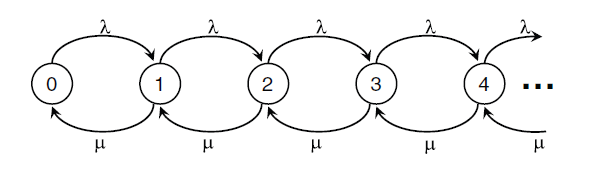
\includegraphics[height=4.5cm]{Rate_transition_diagram.png}
\caption{Rate transition diagram for M/M/1 queue}
\end{figure}

To solve above equations for $\{ p_n \}$, we can use the \textbf{Method of Operators}.
\\ The equations \ref{long_n} and \ref{long_0} can be rewritten as
\begin{eqnarray}
 p_{n+1} &=& \frac{\lambda + \mu}{\mu}p_n  - \frac{\lambda}{\mu} p_{n-1} \label{long_n1} \\
 p_1 &=& \frac{\lambda}{\mu}p_0 \label{long_01}
\end{eqnarray}

Let $\rho = \lambda / \mu$, then \ref{long_n1} becomes
\begin{equation}
    p_{n+1} = (\rho + 1) p_n - \rho p_{n-1} \label{long_n2}
\end{equation}

We define a linear operator $D$ on $\{ p_n \}$ such that
\begin{center}
    $D p_n = p_{n+1}$ \hspace{3mm} and in turn, \\
    $D^m p_n = p_{n+m}$
\end{center}

Writing \ref{long_n} with $n = n+1$ and putting every term on LHS, we get
\begin{center}
    $\mu p_{n+2} - (\lambda + \mu)p_{n+1} + \lambda p_n = 0$ \hspace{5mm} (n $\ge$ 0) \\
\end{center}
Converting to linear operator form, we have
\begin{equation}
    [\mu D^2 - (\lambda + \mu)D + \lambda] p_n = 0 \label{op1}
\end{equation}
subj. to boundary conditions \ref{long_01} and $\sum_{n=0}^{\infty} p_n = 1$
Solving \ref{op1} gives $\{ p_n \}$ as the solution.
On factorizing \ref{op1}, we get
\begin{center}
    $(D-1)(\mu D - \lambda)p_n = 0,$
\end{center}
\begin{center}
and so the final form of $p_n$ is
    $p_n = k_1 (1)^n + k_2 \rho ^n = k_1 + k_2 \rho ^n$
\end{center}
The stability condition for queues requires $\rho < 1$ and as $\sum_{n=0}^{\infty} p_n = 1$, $k_1$ has to be 0, otherwise the summation will go to infinity. Also, from \ref{long_01} and $p_1 = k_2 \rho$, we have $k_2 = p_0$. Hence, $p_n = p_0 \rho ^n$.
Summing $\{ p_n \}$ over all $n$ gives $p_0 = 1 - \rho$.

Now, we find the expected number of customers in the queue in steady state,
Let L denote the value, then
\begin{center}
   $L = \sum_{n=0}^{\infty} n p_n = (1- \rho)\sum_{n=0}^{\infty} n \rho^n$
\end{center}
As $\sum_{n=1}^{\infty}\rho^n = \frac{\rho}{1 - \rho}$, and the derivative of it is $\sum_{n=1}^{\infty}n\rho^{n-1}$, we write $L$ as $(1- \rho)\rho \sum_{n=1}^{\infty}n\rho^{n-1}$.
As $\rho < 1$,
\begin{center}
    $L = (1- \rho)\rho \sum_{n=1}^{\infty}n\rho^{n-1} = (1- \rho) \rho \frac{d}{d \rho}(\frac{\rho}{1- \rho}) = \frac{\rho}{1 - \rho}.$
\end{center}

\begin{center}
$=> L = \frac{\lambda}{\mu - \lambda}$
\end{center}
Using Little's Law ($L = \lambda W$), we get,
\begin{center}
	 $W = \frac{L}{\lambda} = \frac{1}{\mu - \lambda}$
\end{center}
\end{proof}
\vspace{20mm}


\section{Multitype $M/M/1$ queue}
In a multitype $M/M/1$ queue, each customer is of a type $t \in \mathcal{T} := \{1,\ldots T\}$. The arrival rate of customer of type $t$ is a Poisson process with rate $\lambda(t)$ and the service time of the queue is exponential with rate $\mu$. For the queue to be stable, we must have $\rho := \sum_{t\in\mathcal{T}} \rho(t) < 1$, where $\rho(t) := \lambda(t)/\mu$.

We denote the state of queue by vector
$\mathbf{t}=\left(t(1),t(2),\ldots,t(n)\right)$ where $n$ is the number of customers in queue and $t(p)$ is the type of customer at position $p \in \{1,\ldots ,n\}$.

Let $\mathbf{T} = \left\{\mathbf{t}_i : \mathbf{t}_i = \left(t(1),\ldots,t(n)\right), \; t(a)\in\mathcal{T}, \;a\in\left\{1,\ldots,n\right\}, \; n \in \mathbb{N}_0\right\}$. The Markov chain recording the evolution of state has the transition probability
function given by,
\[
q(\mathbf{t},\mathbf{t}') = \begin{cases}
\lambda(t) &\text{if} \; \mathbf{t}'=\left(t(1),\ldots,t(n),t\right)\\
\mu        &\text{if} \; \mathbf{t}'=\left(t(2),\ldots,t(n)\right) 
\end{cases}
\]
The equilibrium distribution of the Markov Chain is
\[
\pi(\mathbf{t}) = (1-\rho)\prod_{a=1}^{n}\rho\left(t(a)\right)
\]


% \begin{corollary}
% A corollary to the theorem is....
% \end{corollary}

% \begin{remark}
% Some remark.......
% \end{remark}


% You may have to type many equations inside the text.  The equation can be typed as below.
% \begin{equation}\label{eqn1}
% f(x) = \frac{x^2-5x+2}{e^x - 2} = {y^5-3 \over e^x-2} %\nonumber
% \end{equation}

% This can be referred as (\ref{eqn1}) and so on.....

% You may have to type a set of equations.  For this you may proceed as given below.
% \begin{eqnarray}
% f(x) &=& e^{1+2(x-a)} + \ldots   \nonumber   \\
%   &=& \log(x+a) + \sin(x+y) + \cdots  \label{eqn2}
% \end{eqnarray}

% % Note: \nonumber will suppress the eqn number in the above.
% % You can type comments like this starting with % as here.

% You may have to cite the articles.  You may do so as \cite{laan} and so on.....
% Note that you have already created the `bib.bib' file and included the entry with the above name. Only
% then you can cite it as above.

\section{Game Theory}
\begin{definition}
A Strategic Game is a model in which 2 or more "players" or "Decision Makers" (DMs) each have a set of "actions" they can choose to perform. These players' actions are interlinked with each other in the way that the outcome for each player is also dependant on the choice of action by the other players. The model also consists of the preferences of each player based on the actions of all players, known as strategy profile.
\end{definition}

\begin{example}
Two competing companies A and B selling the same product may choose to advertise their product or not. If A and B both advertise which includes the cost of advertising, then their earnings would be Rs.10000 per day which includes the cost of advertising. 
If only one of them advertises, then they will earn Rs.15000 while the other would get Rs.7000 earning.
If none of them advertise, then both would save money on advertising and earn Rs.12000 each. The earnings or payoffs of their actions can be modeled as in table \ref{tab:game1}.

\begin{table}[]
    \centering
    \begin{tabular}{c|c|c|}
         & Ad & No Ad \\
         \hline
        Ad & 10000,10000 & 15000, 7000 \\
        No Ad & 7000,15000 & 12000,12000
    \end{tabular}
    \caption{Caption}
    \label{tab:game1}
\end{table}

This is an example of a strategic game where A and B have to decide the perform an action (Advertise or not) and the outcome depends on the actions of all players (A and B in this case).

\end{example}

\begin{definition}
For a strategic game with $N$ players, each having a set of actions 
$ A_i (i \in \{ 1, 2, \ldots, N \} ) $, an action profile 
$a = \{ a_1, a_2, \ldots , a_n \} \in A_1 \times A_2 \times \ldots \times A_N$ is said to be a \textit{Nash Equilibrium} if, for each player $i$, $a_i$ is the best action for them given the actions of all other players. \\
The best action here is based on a payoff function $u_i : A_1 \times A_2 \times \ldots \times A_N \longrightarrow \mathbb{R}$ which each player $i$, has to maximize(or minimize).

In other words, for each player $i$, $a = \{ a_1, a_2, \ldots , a_N \}$ is a Nash Equilibrium if
% \qquad  \quad \; \, ~
\[
u_i(a) \ge u_i(a_{-i}, a_i' ) \qquad \forall \; a_i' \in A_i
\]
where $a_{-i} = \{ a_1, a_2, \ldots , a_{i-1}, a_{i+1}, \ldots , a_N \}$

\end{definition}

\begin{definition}
If the player $i$ has some strategy $a_i$ such that for all possible strategies/actions of other players, $a_i$ fives the best possible outcome for $i$, then $a_i$ is a \textit{dominant strategy} for $i$.

Precisely,
\[
u_i(a_{-i}, a_i) \ge u_i(a_{-i}, a_i') \qquad \forall a_i' \in A_i, \forall a_{-i} \in A_1 \times \ldots \times A_{i-1} \times A_{i+1} \times \ldots \times A_N
\]
\end{definition}


\begin{definition}
Best response function For a player i, the best response function 
$B_i : A_1\times A_2 \times \ldots \times A_{i-1}\times A_{i+1} \times \ldots \times A_n \rightarrow A_i$ is a function that takes the actions of all players other than $i$ and gives a set of actions from $A_i$ which give the maximum value of payoff function for $i$.
So,
\[
B_i(a_{-i}) = \{a_i \in A_i | u_i(a_i,a_{-i})\ge u_i(a_i',a_i) \; \forall \, a_i' \in A_i\}
\]
\end{definition}

\begin{definition}
In pure strategy, each player has to choose an action from with probability
1. So a pure strategy, Nash equilibrium would be an action profile where
each player has exactly one of their possible actions.
\end{definition}

\begin{definition}
In mixed strategy games a player assigns a probability distribution to
their set of actions. A Nash equilibrium would consist of the set of 
probability distributions on the actions of the players so that expected payoff of any player cannot be increased by a change in strategy by just 
them
\end{definition}
